\section{Introduction}
In this section the workflow and results of the Inspection Evaluation are presented and discussed.

The task was to act as experts to evaluate the quality and usability of a website assigned by the evaluators of the course. What follows is an introduction to the content of the website, then the heuristics used are presented, with the agreement on the scale and scores used. A comment on the results is finally presented.

The website has been preliminary checked. A series of question, if not already provided, have been drafted for a set of heuristics to assess. A form has been created to collect the scores by each reviewer. Finally scores and comments have been checked to discover critical flaws or issues with the website.
% TODO Talk about the general method and steps followed - How the study was conducted

\section{Overview of the Website}
The website assigned for the June/July call is \underline{\url{www.unicef.org}}.

UNICEF, or the United Nations Children’s Fund, is a United Nations agency responsible for providing humanitarian and developmental aid to children worldwide. Founded in 1946, UNICEF’s mission is to advocate for the protection of children’s rights, to help meet their basic needs, and to expand their opportunities to reach their full potential. UNICEF operates in over 190 countries and territories, focusing on areas such as child protection, education, immunization, healthcare, nutrition, and emergency relief.

The website presents a virtually infinite amount of information about the activity of the Agency: it presents News and Stories regarding the initiatives taken; Programs addressing various field, Donations which fund the organization; Resources to get involved as a volunteer or worker.

\section{Heuristics}
\textbf{Usability inspection} is the name for a set of methods where an evaluator inspects a user interface.
The evaluation is enabled by the application of the so called Heuristic-driven evaluation technique, a set of principles and checklists that focus on various areas to help discovering potential flaws and issues.


\subsection{Nielsen}
Nielsen heuristics, formulated by Jakob Nielsen, are a set of ten general principles for user interface design, introduced in 1989, updated in 1994, finalized in 2005. They are widely used as guidelines for evaluating and improving the usability of a system.
\begin{enumerate}
	\item \textbf{N1 Visibility of system status} Are the states of the on-going processes of the website always clear? Does the website provide breadcrumbs to define the user position? Does the website use visual elements to highlight user interaction?
	\item \textbf{N2 Match between system and the real world} Does the website use understandable language for its main functionalities? Does the website include icons and assets that are familiar and resemble the real world?
	\item \textbf{N3 User control and freedom} Does the website allow the user to revert or cancel an action? Does the website allow the user to correctly navigate back to a previous section or page? Does the website allow the user to close additional windows at all times?
	\item \textbf{N4 Consistency and standards} Is the website consistent with wording, visual and routing elements? Is the placement of the main components consistent throughout different pages?
	\item \textbf{N5 Error prevention} Are user's inputs, when required, checked for correctness? Does the website provide options to insert information in a guided manner?
	\item \textbf{N6 Recognition rather than recall} Are the website's commands and functionalities visible or easily retrievable when needed? Does the website suggest a set of options to select from for navigation?
	\item \textbf{N7 Flexibility and efficiency of use} Does the website offer shortcuts to common functions? Does the website allow customization and personalization of interaction, catering to both expert and novice users?
	\item \textbf{N8 Aesthetic and minimalist design} Is the website exempt from unnecessary information or links? Are aesthetic choices prioritizing the core elements of the website?
	\item \textbf{N9 Help users recognize, diagnose and recover from errors} Does the website present errors in a user-friendly manner? Does an error state of the website give clear instructions on how to fix/recover from it?
	\item \textbf{N10 Help and documentation} Is the documentation of the website, when provided, searchable and navigable?
\end{enumerate}

It should be noted that the questions are the result of a meeting in which the inspectors brainstormed questions that would answer the given heuristics and agreed the final ones presented in this document.

\subsection{MiLe (Milan Lugano)}
The MiLE heuristics are an extension of Nielsen’s original heuristics, tailored to address specific issues related to web usability. Each heuristics tries to answer given questions (that are shown in the following list). Only a subset of the 40+ heuristics has been used.
\begin{enumerate}
	\item \textbf{Content subset}
		\begin{enumerate}
			\item \textbf{MC1 Information overload} Is the information in a page too much or too little?
			\item \textbf{MC2 Consistency of page content structure} Do pages that present topics of the same category have the same types of elements?
			\item \textbf{MC3 Contextualized information} Do the pages include information that help users understand where they are?
			\item \textbf{MC4 Content organization (hierarchy)} Is the hierarchical organization of topics appropriate for the topics relevance?
		\end{enumerate}

	\item \textbf{Navigation/Interaction subset}
		\begin{enumerate}
			\item \textbf{MN1 Interaction consistency} Do pages of the same type have the same navigation links and interaction capability?
			\item \textbf{MN2 Group navigation-1} It is easy to navigate from/among groups of “items”, and within the items?
			\item \textbf{MN3 Group navigation-2} Do menus create Cognitive Overload?
			\item \textbf{MN4 Structural navigation} Is it easy to navigate among the “components” (“parts”) of a topic?
			\item \textbf{MN5 Semantic navigation} Is it easy to navigate from a topic to a related one (in both directions)?
			\item \textbf{MN6 Landmarks} Are “Landmarks” effective for the user to reach the “key” (most relevant) parts of the web site?
		\end{enumerate}

	\item \textbf{Presentation subset}
		\begin{enumerate}
			\item \textbf{MP1 Text layout} Is the text readable? Is the font size appropriate?
			\item \textbf{MP2 Interaction placeholders-semiotics} Interactive elements are “intuitive”?
			\item \textbf{MP3 Interaction placeholders-consistency} Textual or visual labels of interactive elements are consistent in terms of wording, shape, color, position, etc.
			\item \textbf{MP4 Consistency of Visual Elements} In pages of the same type do visual elements have the same visual properties?
			\item \textbf{MP5 Hierarchy-1} Is the on-screen allocation of contents within a page appropriate for their relevance?
			\item \textbf{MP6 Hierarchy-2} Is the on-screen allocation of visual elements appropriate for their relevance?
			\item \textbf{MP7 Spatial allocation-1} Are “Semantically related” elements close to each other?
			\item \textbf{MP8 Spatial allocation-2} Are "Semantically distant” element placed distant from each other?
			\item \textbf{MP9 Consistency of Page Spatial Structure} Do pages of the same type have the same spatial organization for the various visual elements?
		\end{enumerate}
\end{enumerate}

\section{Execution of the inspection}
\subsection{Inspection Sheet}
An inspection sheet (in the form of a Google Form) was used to collect the scores and comments from each inspector. The form has been divided into sections (as shown in Figures \ref{fig:nielsenForm} and \ref{fig:mileForm}) in representing the current subset of Heuristics being used to evaluate the website: Nielsen; MiLE: Content; MiLE: Navigation; MiLE: Presentation. Each section contains a subsection per-heuristics, which in turns contain a input field for each of the questions that are linked to the current heuristic. Next to each question a field to add comments about the score is also provided.

\subsection{Scale used}
The scale that was agreed among inspectors is the 1-5 scale, where:
\begin{itemize}
	\item 1 represents \textit{Strongly disagree}
	\item 5 represents \textit{Strongly agree}
\end{itemize}
Adding more granularity to the choice by means of the 1-10 scale would make inspection and results' evaluation more harder, so the 1-5 scale felt like a good balance between quality and simplicity of the evaluation for its inspectors.
Finally, each question has been made not-mandatory to manage such cases in which an inspector would realize a given question or heuristic was not applicable in the context of the UNICEF website.

\begin{figure}[h]
	\centering
	\includegraphics[width=0.6\textwidth]{img/nielsen_heuristics_form.png}
	\caption{Nielsen's Heuristics' section on the Inspection form}
	\label{fig:nielsenForm}
\end{figure}

\begin{figure}[h]
	\centering
	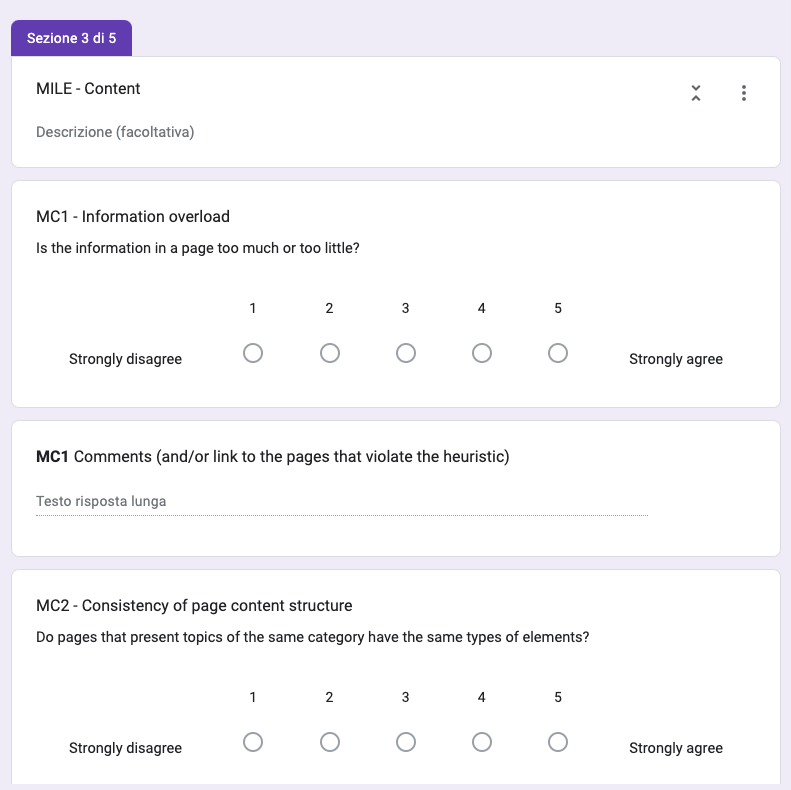
\includegraphics[width=0.6\textwidth]{img/mile_content_form.png}
	\caption{MiLE Content Heuristics' section on the Inspection form}
	\label{fig:mileForm}
\end{figure}

\subsection{Constraints on the inspection}
To maintain consistency in the evaluation of the heuristic throughout different pages, the group agreed that a better suited option would be to evaluate a category of heuristics on multiple pages at the time. Given the size of the website to evaluate, so the difficulty in defining a proper amount of pages to visit (per heuristic), we decided to set that amount at approximately 50 pages. Also time constraints were not imposed.

It should be noted that various sub-websites (such as the one to file an application for a career within UNICEF, the Donation website etc.) are presented throughout the main website. Such websites were ignored during the evaluation. The group decided to focus on websites that would provide knowledge and content regarding the Agency activity, rather than evaluating applications which represent a really small part of the entire website.

\pagebreak

\section{Final scores}
After the Inspection phase, we reviewed the scores and discussed the results. The group decided to define the final scores as the averages of the partial scores and also defined a baseline over which the score would be considered acceptable. A score being over a baseline of \textbf{2,5} would mean that no further investigation would explicitly target the associated heuristic or question.

Tables \ref{tab:N_final_scores}, \ref{tab:MC_final_scores}, \ref{tab:MN_final_scores}, \ref{tab:MP_final_scores} show the final scores for each heuristic and question:


\begin{longtable}{|p{0.7\linewidth}|p{0.2\linewidth}|}
    \caption{Nielsen's Heuristics' Final Scores} \label{tab:N_final_scores}\\
    \hline
    \multicolumn{2}{|c|}{\textbf{Nielsen's Heuristics' Final Scores}} \\
    \hline
    \textbf{Question} & \textbf{Final Score} \\
    \hline
    \endfirsthead
    \multicolumn{2}{c}%
    {\tablename\ \thetable\ -- \textit{Continued from previous page}} \\
    \hline
    \multicolumn{2}{|c|}{\textbf{Nielsen's Heuristics' Final Scores}} \\
    \hline
    \textbf{Inspector} & \textbf{Score} \\
    \hline
    \endhead
    \endfoot
    \hline
    \endlastfoot

\multicolumn{2}{|l|}{\textbf{N1 Visibility of system status}} \\
\hline
Are the states of the on-going processes of the website always clear? & 4,25  \\
\hline
Does the website provide breadcrumbs to define the user position? & \textbf{2,5} \\
\hline
Does the website use visual elements to highlight user interaction? & 3,75 \\
\hline

\multicolumn{2}{|l|}{\textbf{N2 Match between system and the real world}} \\
\hline
Does the website use understandable language for its main functionalities? & 4,5  \\
\hline
Does the website include icons and assets that are familiar and resemble the real world? & 4,25 \\
\hline

\pagebreak

\multicolumn{2}{|l|}{\textbf{N3 User control and freedom}} \\
\hline
Does the website allow the user to revert or cancel an action? & 4  \\
\hline
Does the website allow the user to correctly navigate back to a previous section or page? & \textbf{2} \\
\hline
Does the website allow the user to close additional windows at all times? & 5 \\
\hline

\multicolumn{2}{|l|}{\textbf{N4 Consistency and standards}} \\
\hline
Is the website consistent with wording, visual and routing elements? & \textbf{1,75}  \\
\hline
Is the placement of the main components consistent throughout different pages? & 3,5 \\
\hline

\multicolumn{2}{|l|}{\textbf{N5 Error prevention}} \\
\hline
Are user's inputs, when required, checked for correctness? & 3,75  \\
\hline
Does the website provide options to insert information in a guided manner? & 3,5 \\
\hline

\multicolumn{2}{|l|}{\textbf{N6 Recognition rather than recall}} \\
\hline
Are the website's commands and functionalities visible or easily retrievable when needed? & 3,75  \\
\hline
Does the website suggest a set of options to select from for navigation? & 4 \\
\hline

\multicolumn{2}{|l|}{\textbf{N7 Flexibility and efficiency of use}} \\
\hline
Does the website offer shortcuts to common functions? & \text{2,5}  \\
\hline
Does the website allow customization and personalization of interaction, catering to both expert and novice users? & \textbf{1,33333} \\
\hline

\multicolumn{2}{|l|}{\textbf{N8 Aesthetic and minimalist design}} \\
\hline
Is the website exempt from unnecessary information or links? & \textbf{1,75}  \\
\hline
Are aesthetic choices prioritizing the core elements of the website? & 3 \\
\hline

\multicolumn{2}{|l|}{\textbf{N9 Help users recognize, diagnose and recover from errors}} \\
\hline
Does the website present errors in a user-friendly manner? & 3,25  \\
\hline
Does an error state of the website give clear instructions on how to fix/recover from it? & 3 \\
\hline

\multicolumn{2}{|l|}{\textbf{N10 Help and documentation}} \\
\hline
Is the documentation of the website, when provided, searchable and navigable? & 2,5  \\
\hline

\end{longtable}

\begin{longtable}{|p{0.7\linewidth}|p{0.2\linewidth}|}
    \caption{MiLE (Content) Heuristics' Final Scores} \label{tab:MC_final_scores}\\
    \hline
    \multicolumn{2}{|c|}{\textbf{MiLE (Content) Heuristics' Final Scores}} \\
    \hline
    \textbf{Question} & \textbf{Final Score} \\
    \hline
    \endfirsthead
    \multicolumn{2}{c}%
    {\tablename\ \thetable\ -- \textit{Continued from previous page}} \\
    \hline
    \multicolumn{2}{|c|}{\textbf{MiLE (Content) Heuristics' Final Scores}} \\
    \hline
    \textbf{Inspector} & \textbf{Score} \\
    \hline
    \endhead
    \endfoot
    \hline
    \endlastfoot

\multicolumn{2}{|l|}{\textbf{MC1 Information overload}} \\
\hline
Is the information in a page too much or too little? & 3,75  \\
\hline

\multicolumn{2}{|l|}{\textbf{MC2 Consistency of page content structure}} \\
\hline
Do pages that present topics of the same category have the same types of elements? & 2,75  \\
\hline

\multicolumn{2}{|l|}{\textbf{MC3 Contextualized information}} \\
\hline
Do the pages include information that help users understand where they are? & 2,75  \\
\hline

\multicolumn{2}{|l|}{\textbf{MC4 Content organization (hierarchy)}} \\
\hline
Is the hierarchical organization of topics appropriate for the topics relevance? & 3  \\
\hline

\end{longtable}

\begin{longtable}{|p{0.7\linewidth}|p{0.2\linewidth}|}
    \caption{MiLE (Navigation) Heuristics' Final Scores} \label{tab:MN_final_scores}\\
    \hline
    \multicolumn{2}{|c|}{\textbf{MiLE (Navigation) Heuristics' Final Scores}} \\
    \hline
    \textbf{Question} & \textbf{Final Score} \\
    \hline
    \endfirsthead
    \multicolumn{2}{c}%
    {\tablename\ \thetable\ -- \textit{Continued from previous page}} \\
    \hline
    \multicolumn{2}{|c|}{\textbf{MiLE (Navigation) Heuristics' Final Scores}} \\
    \hline
    \textbf{Inspector} & \textbf{Score} \\
    \hline
    \endhead
    \endfoot
    \hline
    \endlastfoot

\multicolumn{2}{|l|}{\textbf{MN1 Interaction consistency}} \\
\hline
Do pages of the same type have the same navigation links and interaction capability? & \textbf{1,66667}  \\
\hline

\multicolumn{2}{|l|}{\textbf{MN2 Group navigation-1}} \\
\hline
It is easy to navigate from/among groups of “items”, and within the items? & \textbf{2}  \\
\hline

\multicolumn{2}{|l|}{\textbf{MN3 Group navigation-2}} \\
\hline
Do menus create Cognitive Overload? & 3,66667  \\
\hline

\multicolumn{2}{|l|}{\textbf{MN4 Structural navigation}} \\
\hline
Is it easy to navigate among the “components” (“parts”) of a topic? & 2,66667  \\
\hline

\multicolumn{2}{|l|}{\textbf{MN5 Semantic navigation}} \\
\hline
Is it easy to navigate from a topic to a related one (in both directions)? & 3  \\
\hline

\multicolumn{2}{|l|}{\textbf{MN6 Landmarks}} \\
\hline
Are “Landmarks” effective for the user to reach the “key” (most relevant) parts of the web site? & 3  \\
\hline

\end{longtable}

\begin{longtable}{|p{0.7\linewidth}|p{0.2\linewidth}|}
    \caption{MiLE (Presentation) Heuristics' Final Scores} \label{tab:MP_final_scores}\\
    \hline
    \multicolumn{2}{|c|}{\textbf{MiLE (Presentation) Heuristics' Final Scores}} \\
    \hline
    \textbf{Question} & \textbf{Final Score} \\
    \hline
    \endfirsthead
    \multicolumn{2}{c}%
    {\tablename\ \thetable\ -- \textit{Continued from previous page}} \\
    \hline
    \multicolumn{2}{|c|}{\textbf{MiLE (Presentation) Heuristics' Final Scores}} \\
    \hline
    \textbf{Inspector} & \textbf{Score} \\
    \hline
    \endhead
    \endfoot
    \hline
    \endlastfoot

\multicolumn{2}{|l|}{\textbf{MP1 Text layout}} \\
\hline
Is the text readable? Is the font size appropriate? & 5  \\
\hline

\multicolumn{2}{|l|}{\textbf{MP2 Interaction placeholders-semiotics}} \\
\hline
It is easy to navigate from/among groups of “items”, and within the items? & 4,66667  \\
\hline

\multicolumn{2}{|l|}{\textbf{MP3 Interaction placeholders-consistency}} \\
\hline
Textual or visual labels of interactive elements are consistent in terms of wording, shape, color, position, etc. & 3  \\
\hline

\multicolumn{2}{|l|}{\textbf{MP4 Consistency of Visual Elements}} \\
\hline
In pages of the same type do visual elements have the same visual properties? & 3  \\
\hline

\multicolumn{2}{|l|}{\textbf{MP5 Hierarchy-1}} \\
\hline
Is the on-screen allocation of contents within a page appropriate for their relevance? & 4,33333  \\
\hline

\multicolumn{2}{|l|}{\textbf{MP6 Hierarchy-2}} \\
\hline
Is the on-screen allocation of visual elements appropriate for their relevance? & 4  \\
\hline

\multicolumn{2}{|l|}{\textbf{MP7 Spatial allocation-1}} \\
\hline
Are “Semantically related” elements close to each other? & 4,66667  \\
\hline

\multicolumn{2}{|l|}{\textbf{MP8 Spatial allocation-2}} \\
\hline
Are "Semantically distant” element placed distant from each other? & 4,5  \\
\hline

\multicolumn{2}{|l|}{\textbf{MP9 Consistency of Page Spatial Structure}} \\
\hline
Do pages of the same type have the same spatial organization for the various visual elements? & 3  \\
\hline

\end{longtable}

\section{Data Analysis - Aggregate}
PROVIDE AGGREGATED DATA, e.g., MEAN VALUES FOR ALL Heuristics,
(MEAN) SCORE BY DIMENSIONS (e.g., for CONTENT HEURISTICS,
NAVIGATION HEURISTICS, ect.)

\section{Screenshots}

\section{Conclusions}
The UNICEF website has the purpose to deliver as much information and details possible about the activity of this Agency to its readers for transparency in the operations and actions taken. Another goal is to convince potential new and recurring donators to help with UNICEF's cause and inspire the next generation of volunteers and workers at this agency.

The sheer amount of content provided is not properly organized so the user could easily get lost while surfing this website. The content is often not separated into proper sections, sub-websites make usability a nightmare and apparently no guidelines exist to define what links and buttons should point to or do. Breadcrumbs are not correctly used (if they are presented anyway) and the user could get easily lost into the ocean of content.

% TODO include somehow
From the results, it's clear that the main problems is the many ways in which many informations are presented and the ways in which these information can be reached. The additional problem is that many times the content is pages at different levels even though these levels are supposed to be the same.
